\chapter{Applikationslaget}
Applikationslaget er det lag af software i det samlede distribuerede system, som installeres eller afvikles hos brugeren. Applikationslaget er designet til at være platformuafhængigt, jf. systemets arkitektur. Derved er lagets model- og præsentationslag designet til at være portabelt, hvorimod view-laget er platformspecifikt. 

Som følge af multi-lag arkitekturen kunne applikationslaget samt de platform-specifikke view-implementeringer
designes, uafhængigt af hinanden, så længe interfaces blev specificeret undervejs i processen. 

Presenter interfacet specificerer hvilke metoder og hvilken funktionalitet et view skal have.
Her ses klassediagrammet for ISignUpView.

\begin{figure}
\centering
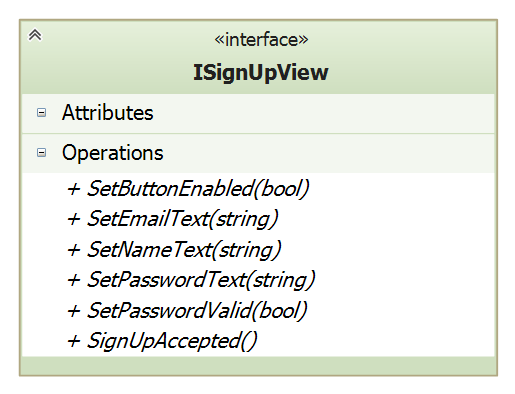
\includegraphics[width=0.35\linewidth]{figs/design/application_isignupview}
\caption{ISignUpView}
\label{fig:application_isignupview}
\end{figure}
View'et i hver applikation implementerer interfacet og opretter en controller, hvis interface ses nedenfor.
Interfacet indeholder de funktioner user stories'ne leder op til.
\begin{figure}
\centering
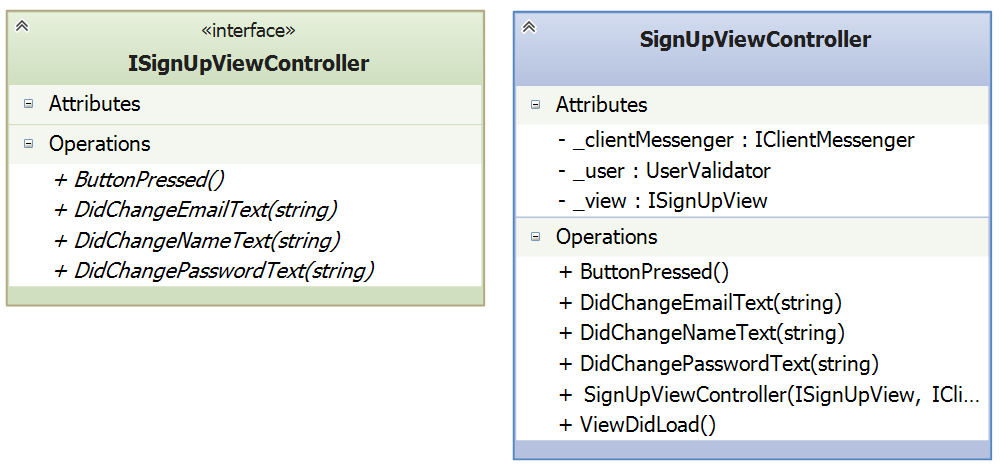
\includegraphics[width=0.7\linewidth]{figs/design/application_signupviewcontrollerandinterface}
\caption{ISignUpViewController og SignUpViewController}
\label{fig:application_isignupviewcontroller}
\end{figure}
Figur~\ref{fig:application_isignupviewcontroller} viser også SignUpViewController's konkrete klasse, der indeholder flere metoder og attributter, som måden MVP er lavet i applikationslaget viste sig at kræve.
Det er attributter som \_clientMessenger, som er klienten, der kommunikerer med serveren. 
\_user af typen UserValidater er en klasse i præsentationslaget der er platformsuafhængig til at validere om bruger informationen er gyldig. 

Controlleren kender ISignUpView, så den kalder funktionerne i view'et og på den måde er logik og view adskilt.

Designet af funktionaliteten bag user story'en, der viser nyeste målinger har ført til følgende konkrete controller klasse.

\begin{figure}
\centering
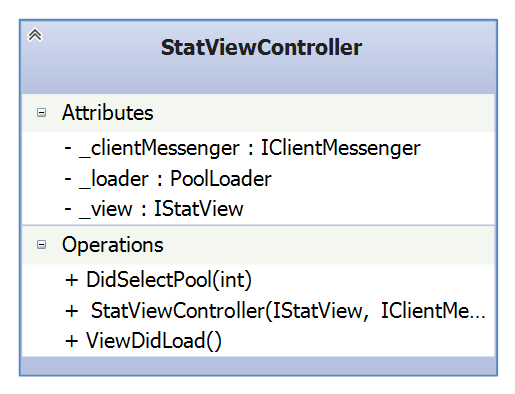
\includegraphics[width=0.35\linewidth]{figs/design/application_statviewcontroller}
\caption{StatViewController konkret klasse}
\label{fig:application_statviewcontroller}
\end{figure}

For yderligere forklaring se dokumentation afsnit Applikationslaget under Design.

\subsection{Windows GUI}
I Windows applikationen designes view-klasser, der implementerer view-interfacet defineret i præsentationslaget.
Designet af Windows GUI er lavet således, at codebehind filerne implementerer hver sit view-interfacet fra præsentationslaget. Codebehind agerer dermed som en bro, i mellem Smartpools præsentationslag, og WPF view-lag.

I klasse diagrammet nedenfor, ses Windows designet, af WinCreateUserView der implementerer ISignUpView fra applikationslaget og har en SignUpViewController.
\begin{figure}
\centering
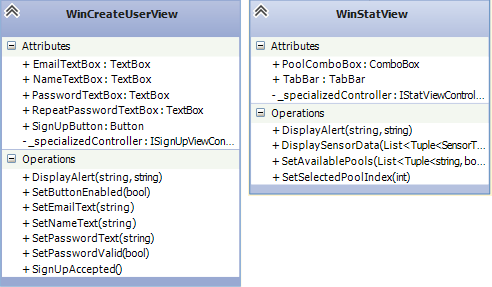
\includegraphics[width=0.7\linewidth]{figs/design/wincreateuserandwinstatviewview}
\caption{WinCreateUserView og WinStatView}
\label{fig:wincreateuserandwinstatviewview}
\end{figure}

Ligeledes er view klassen for WinStatView designet.
Klassen ses på figur~\ref{wincreateuserandwinstatviewview}.

For yderligere forklaring se dokumentation afsnit Applikationslaget under Design.